\resizebox{\textwidth}{!}{
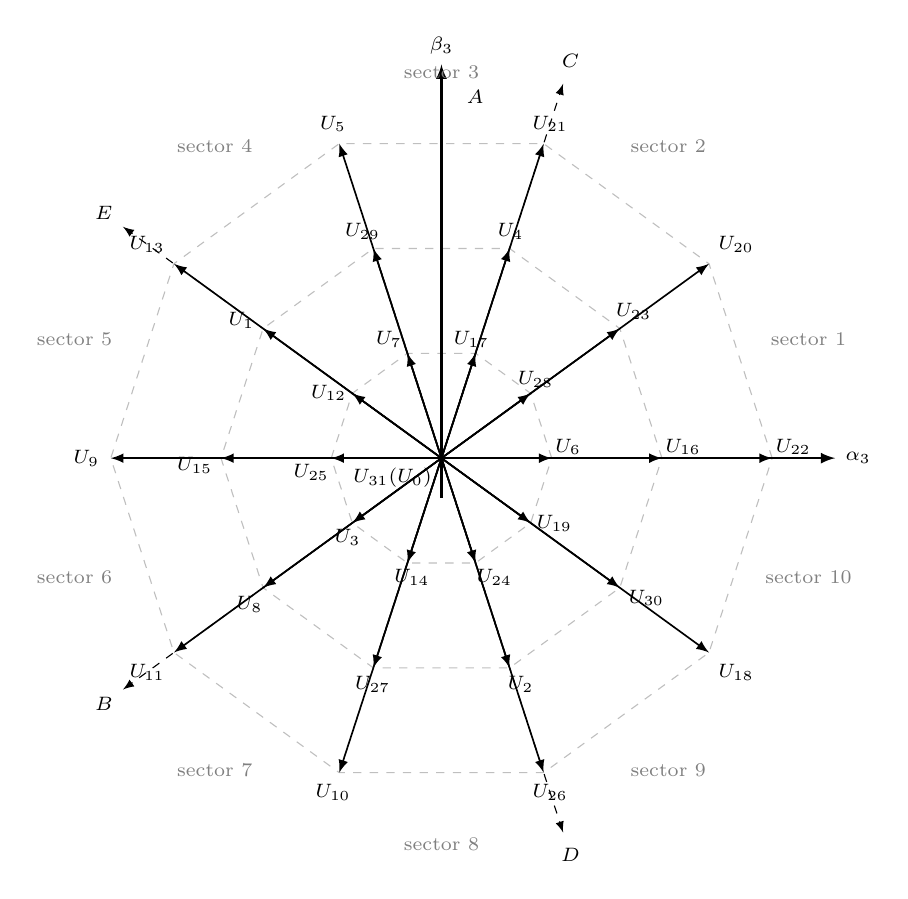
\begin{tikzpicture}[>=latex, font=\scriptsize]

    % Definice poloměrů
    \def\Rone{1.4}   
    \def\Rtwo{2.8}   
    \def\Rthree{4.2} 
    \def\Raxis{5.0}  

    % 1. Kreslení pozadí (čárkované desetiúhelníky)
    \foreach \r in {\Rone, \Rtwo, \Rthree} {
        \draw[dashed, gray!50] (0:\r) \foreach \x in {36,72,...,360} {-- (\x:\r)} -- cycle;
    }

    % 2. Hlavní osy (alfa 3 a beta 3)
    \draw[->, thick] (-0.5,0) -- (\Raxis,0) node[right] {$\alpha_3$};
    \draw[->, thick] (0,-0.5) -- (0,\Raxis) node[above] {$\beta_3$};

    % Středový bod
    \node[below left] at (0,0) {$U_{31}(U_0)$};

    % 3. VEKTORY A POPISKY PRO OBRÁZEK (b)

    % VNĚJŠÍ ÚROVEŇ (Level 3)
    \foreach \ang/\lab in {0/U_{22}, 36/U_{20}, 72/U_{21}, 108/U_{5}, 144/U_{13}, 180/U_9, 216/U_{11}, 252/U_{10}, 288/U_{26}, 324/U_{18}} {
        \draw[->, semithick] (0,0) -- (\ang:\Rthree);
        \ifnum\ang=0
            \node[anchor=south west, inner sep=1pt] at (\ang:\Rthree) {$\lab$};
        \else
            \node[anchor=\ang+180, inner sep=4pt] at (\ang:\Rthree) {$\lab$};
        \fi
    }

    % STŘEDNÍ ÚROVEŇ (Level 2)
    \foreach \ang/\lab in {0/U_{16}, 36/U_{23}, 72/U_4, 108/U_{29}, 144/U_{1}, 180/U_{15}, 216/U_{8}, 252/U_{27}, 288/U_{2}, 324/U_{30}} {
        \draw[->, semithick] (0,0) -- (\ang:\Rtwo);
        \ifnum\ang=0
            \node[anchor=south west, inner sep=1pt] at (\ang:\Rtwo) {$\lab$};
        \else
            \node[anchor=\ang+195, inner sep=3pt] at (\ang:\Rtwo) {$\lab$};
        \fi
    }

    % VNITŘNÍ ÚROVEŇ (Level 1)
    \foreach \ang/\lab in {0/U_6, 36/U_{28}, 72/U_{17}, 108/U_{7}, 144/U_{12}, 180/U_{25}, 216/U_3, 252/U_{14}, 288/U_{24}, 324/U_{19}} {
        \draw[->, semithick] (0,0) -- (\ang:\Rone);
        \ifnum\ang=0
            \node[anchor=south west, inner sep=1pt] at (\ang:\Rone) {$\lab$};
        \else
            \node[anchor=\ang+215, inner sep=2pt] at (\ang:\Rone) {$\lab$};
        \fi
    }

    % 4. Fázové osy pro (b) - A, C, E, B, D
    \node[anchor=north west] at (0.2, \Raxis-0.2) {$A$}; % Label u osy alfa
    \foreach \ang/\name in {72/C, 144/E, 216/B, 288/D} {
        \draw[->, dashed] (0,0) -- (\ang:\Raxis);
        \node at (\ang:\Raxis + 0.3) {$\name$};
    }
    
    % 5. Sektory
    \foreach \s/\ang in {1/18, 2/54, 3/90, 4/126, 5/162, 6/198, 7/234, 8/270, 9/306, 10/342} {
        \node[text=gray] at (\ang:\Rthree + 0.7) {sector \s};
    }



\end{tikzpicture}
}